\documentclass{article}

\usepackage{dirtree}

\usepackage[
  height=9in,      % height of the text block
  width=7.5in,       % width of the text block
  top=78pt,        % distance of the text block from the top of the page
  headheight=48pt, % height for the header block
  headsep=12pt,    % distance from the header block to the text block
  heightrounded,   % ensure an integer number of lines
        % show the main blocks
  verbose,         % show the values of the parameters in the log file
]{geometry}
\setlength{\parindent}{0pt}
\usepackage{amsmath}
\usepackage{courier}
\usepackage{graphicx}
\usepackage{amsmath}
\usepackage{booktabs}
\usepackage{fancyhdr}
\usepackage{float}
\usepackage{mathtools}

\pagestyle{fancy}
\fancyhead[L]{Pattern and Speech Recognition WS1617\\ Assignment 06}
\fancyhead[R]{ Vinh Thinh Ho (2562630) \\ Noshaba Cheema (2562653)}

\renewcommand{\headrulewidth}{0.35pt}
\newcommand\tab[1][1cm]{\hspace*{#1}}

\begin{document}
\section*{Exercise 6.1}
a) False. The true statemet is: "Regularization is any modification we make to a learning algorithm that is intended to reduce its generalization error but \textbf{not} its training error". The reason is regularization is used to overcome over-fitting in learning data set, that is the learned model will minimize the training error, however it is so complex that cannot generalize for the real data. So, we will try to reduce the generalization error at the cost of increasing training error.\\
b) True. We have:
\begin{align*}
y &= log(x^{\alpha_1}e^{\alpha_2})\\
 &= log(x^{\alpha_1}) + log(e^{\alpha_2}\\
  &= \alpha_1 log(x) + \alpha_2
\end{align*}
Hence, we can apply linear regression to learn parameters $\alpha$ for this model.

\section*{Exercise 6.2}
The similarity between bagging and dropout is that both methods are methods to overcome overfitting. However, dropout introduces random noise by essentially switching off a specific percentage of neurons to reduce overfitting, while bagging creates aritificial training subsets of the training data (one subset for one estimator) and then finally takes the average of all estimators, if we are dealing with a regression problem, or the majority vote of all classifiers, if we are dealing with a classification problem.\\
Boosting and bagging are both essamble methods, meaning that both combine the results of different base estimators to improve generalizability / robustness over a single estimator. However, by contrast to bagging, the base estimators in boosting are not built independanlty but sequentially, meaning that one tries to reduce the bias of the combined estimator and hence, boosting combines several weak models to produce one powerful esemble.
%The similarity between bagging and dropout is both methods will try to train the data with different models and then try to use the prediction from these models to get the final prediction. However, while in bagging, models are trained independently, different models in dropout method could share some parameters. Bagging and boosting are both ensemble methods, but there are some differences. For example, goal of bagging is to minimize the variance, but for boosting, it is to improve the predictive force. The methods used to combine single models are also different. Bagging uses weighted average of prediction of individual models, why boosting uses the majority of votes from these models.

\section*{Exercise 6.3}
a) We have:
$$w_j^\tau = \{1 - (1 - \epsilon \lambda_j)^\tau\} w_j^* $$
If $\tau \to \infty$ and $|1 - \epsilon \lambda_j| < 1$, we have:
$$\lim_{\tau \to \infty} w_j^\tau = \lim_{\tau \to \infty}  \{1 - (1 - \epsilon \lambda_j)^\tau\} w_j^* = \{1 - 0\} w^*_j = 1 w^*_j = w^*_j$$
b) We have:
$$\left(\lambda_j \gg (\epsilon \tau)^{-1}\right) \Leftrightarrow \left(\lambda_j \gg \frac{1}{\epsilon \tau}\right) \Leftrightarrow \left(\epsilon \lambda_j \gg \frac{1}{\tau}\right)$$
Since $|1 - \epsilon \lambda_j| < 1$, we have $0 < \epsilon \lambda_j < 2$ and because $\epsilon \lambda_j$ and $\frac{1}{\tau}$ must be positive, we have:
$$2 > \epsilon \lambda_j \gg \frac{1}{\tau} > 0$$
Since $\tau$ are the number of steps and we assume that some number of steps have been done (meaning at least one step), we can say $1 \geq \frac{1}{\tau} > 0$, so $\frac{1}{\tau}$ is at most 1. However, $\frac{1}{\tau}$ should fullfill $2 > \epsilon \lambda_j \gg \frac{1}{\tau} > 0$, which means $\frac{1}{\tau}$ should be much smaller than 2. So we can assume a much smaller number for $\frac{1}{\tau}$, e.g. 0.0001, which would mean that $\tau = 10000$, for example. In that case $(1 - \epsilon \lambda_j)^\tau$ would be again close to 0. Hence, our assumption that $w_j^\tau \simeq w_j^*$ when $\lambda_j \gg (\epsilon \tau)^{-1}$ would be true.\\
\\
On the other hand, if we have:
$$\left(\lambda_j \ll (\epsilon \tau)^{-1}\right) \Leftrightarrow \left(\lambda_j \ll \frac{1}{\epsilon \tau}\right) \Leftrightarrow \left(\epsilon \lambda_j \ll \frac{1}{\tau}\right)$$
And since, $|1 - \epsilon \lambda_j| < 1$ and $0 < \frac{1}{\tau} \leq 1$:
$$0 < \epsilon \lambda_j \ll \frac{1}{\tau} \leq 1$$
So if $\epsilon \lambda_j \ll 1$, then $(1 - \epsilon \lambda_j)$ becomes close to 1.\\
If $\frac{1}{\tau}$ is not very small, meaning that $\tau$ is just a few steps, then $(1 - \epsilon \lambda_j)^\tau$ is still close to 1 and the expression $\{1 - (1 - \epsilon \lambda_j)^\tau\}$ becomes very small, so $|w_j^\tau| \ll |w_j^*|$. If $\frac{1}{\tau}$ is very small, meaning that $\tau$ is a huge amount of steps, then $\epsilon \lambda_j$ is also a lot smaller than $\frac{1}{\tau}$, so the whole expression $(1 - \epsilon \lambda_j)^\tau$ is still close to 1 and $\{1 - (1 - \epsilon \lambda_j)^\tau\}$ becomes very small, so we still have $|w_j^\tau| \ll |w_j^*|$.\\
\\
c)\\
The regularization parameter determines in some way, how close you are to the optimal weights. If $\alpha$ is very small or 0, then you are close to the optimal weights for your training set, which is good for classifying your training data, but bad if you want your model to generalize well. If your weights are too close to the optimal weights for the training set, then that means, that your model is probably overfitted. If you chose a greater value for your regularization parameter $\alpha$, then your weights will be furhter from the optimal weights for your model but it would generalize much better and would probably now have a lower test error.\\
The term $(\epsilon \tau)^{-1}$ works in a similar fashion. If it is small enough that $\lambda_j \gg (\epsilon \tau)^{-1}$, then your weights are close to the optimal weights, which again may be bad, since now your model is overfitted. However, if $\lambda_j \ll (\epsilon \tau)^{-1}$ then, this is similar to chose a bigger value for $\alpha$, since now the weights are less close to the optimal weights for the training set and your model might generalize much better.

\section*{Exercise 6.4}
a) See \textbf{6.4.py}\\
\begin{figure}[ht]
	\centering
	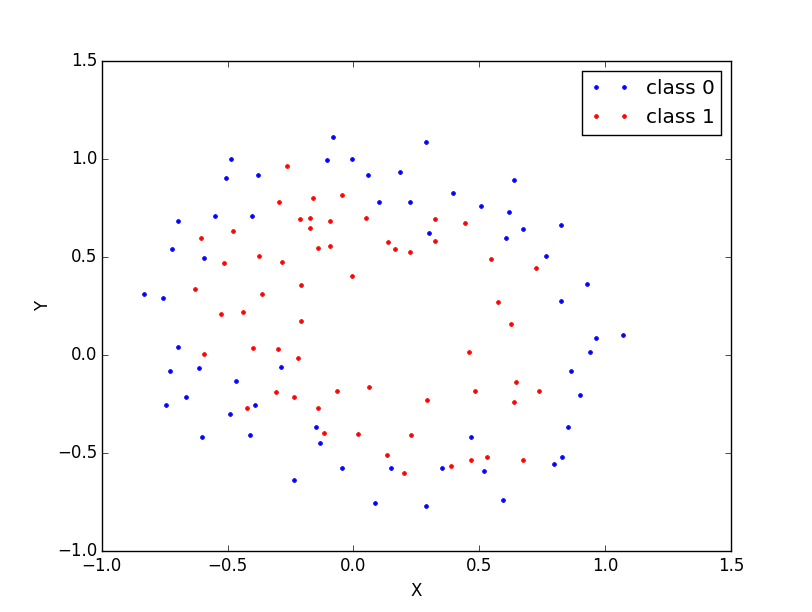
\includegraphics[scale=0.35]{64a.png}
	\caption{data}
\end{figure}

b) See \textbf{6.4.py}\\
c)\\
- Gradient of cost function:\\
We have:
\begin{align*}
\frac{\partial h_\theta(x)}{\partial \theta_i} &= \frac{\partial h_\theta(x)}{\partial (\theta^Tx)}.\frac{\partial (\theta^Tx)}{\partial \theta_i}\\
&= h_\theta(x).(1-h_\theta(x)).x_i
\end{align*}
- Gradient $G \in R^n$ and 
\begin{align*}
G[k] &= \frac{\partial J(\theta)}{\partial \theta_i}\\
&= -\frac{\partial (\frac{1}{m}\sum\limits_{i=1}^{m}[y_i log(h_\theta(x_i))])}{\partial \theta_k}
-\frac{\partial (\frac{1}{m}\sum\limits_{i=1}^{m}[(1 - y_i)log(1-h_\theta(x_i))])}{\partial \theta_k} + \frac{\partial \frac{\lambda}{2m}\sum\limits_{j=1}^{n}\theta_j^2}{\partial \theta_k}\\
&= -\frac{1}{m}\sum\limits_{i=1}^{m}[\frac{y_i}{h_{\theta}(x_i)}h_{\theta}(x_i)(1-h_{\theta}(x_i))x_{i,k}]
-\frac{1}{m}\sum\limits_{i=1}^{m}[\frac{1- y_i}{1- h_{\theta}(x_i)}h_{\theta}(x_i)(1-h_{\theta}(x_i))(-x_{i,k})]
+ \frac{\lambda}{m}\theta_k\\
&= -\frac{1}{m}\sum\limits_{i=1}^{m}[y_i (1-h_{\theta}(x_i))x_{i,k}]
+\frac{1}{m}\sum\limits_{i=1}^{m}[(1- y_i)h_{\theta}(x_i)x_{i,k}]
+ \frac{\lambda}{m}\theta_k\\
&= \frac{1}{m}\sum\limits_{i=1}^{m}[(h_{\theta}(x_i) - y_i)x_{i,k}]
+ \frac{\lambda}{m}\theta_k
\end{align*}
- Hessian matrix of cost function $H \in R^{n \times n}$ and
\begin{align*}
H[k,l] &= \frac{\partial G[k]}{\partial \theta_l}\\
&= \frac{1}{m}\sum\limits_{i=1}^{m}[h_{\theta}(x_i)(1-h_{\theta}(x_i))x_{i,l}x_{i,k}]
+ \frac{\lambda}{m}\frac{\partial\theta_k}{\partial \theta_l}\\
&=  \frac{1}{m}\sum\limits_{i=1}^{m}[h_{\theta}(x_i)(1-h_{\theta}(x_i))x_{i,l}x_{i,k}]\ (if\ k \ne l)\\
or &= \frac{1}{m}\sum\limits_{i=1}^{m}[h_{\theta}(x_i)(1-h_{\theta}(x_i))x_{i,l}x_{i,k}] + \frac{\lambda}{m}\ (if\ k = l)
\end{align*}
d) See \textbf{6.4.py}\\
e)
\begin{figure}[ht]
	\centering
	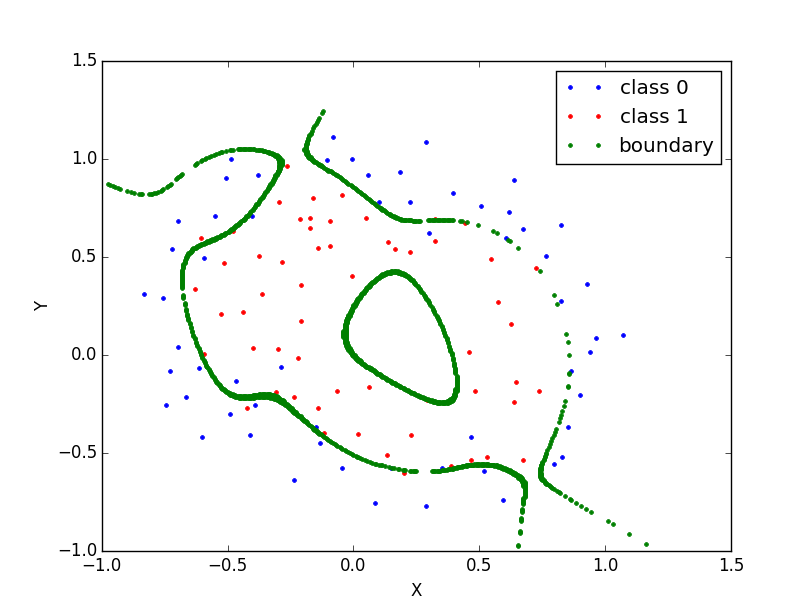
\includegraphics[scale=0.35]{lambda_0.png}
	\caption{$\lambda = 0$}
\end{figure}
\begin{figure}[ht]
	\centering
	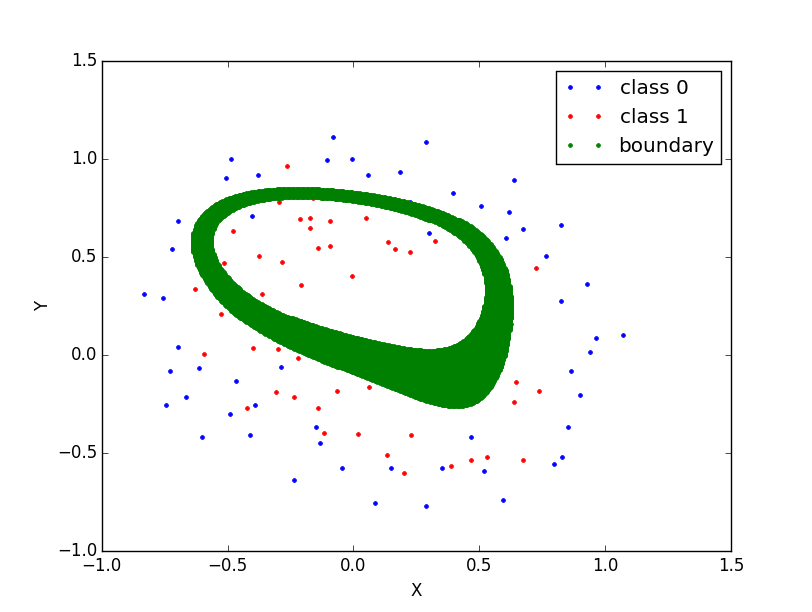
\includegraphics[scale=0.35]{lambda_1.png}
	\caption{$\lambda = 1$}
\end{figure}
\begin{figure}[ht]
	\centering
	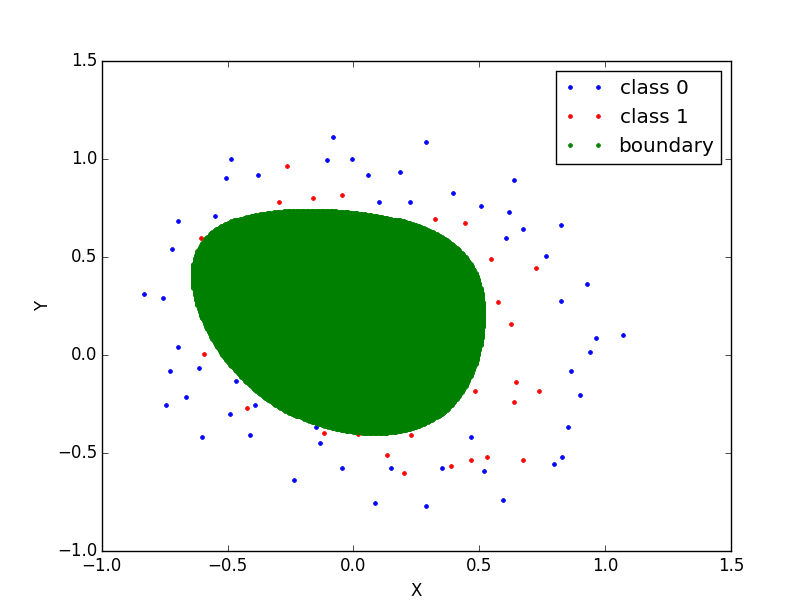
\includegraphics[scale=0.35]{lambda_10.png}
	\caption{$\lambda = 10$}
\end{figure}
\newpage
We can see that the plot with $\lambda = 0$ perfectly separate the data, but seem a little bit overfit. With $\lambda = 1$, the model slightly underfit the data, and with $\lambda = 10$, the model significantly underfit the data.

We tuned $\lambda$ and below is the plot with $\lambda = 0.01$
\begin{figure}[ht]
	\centering
	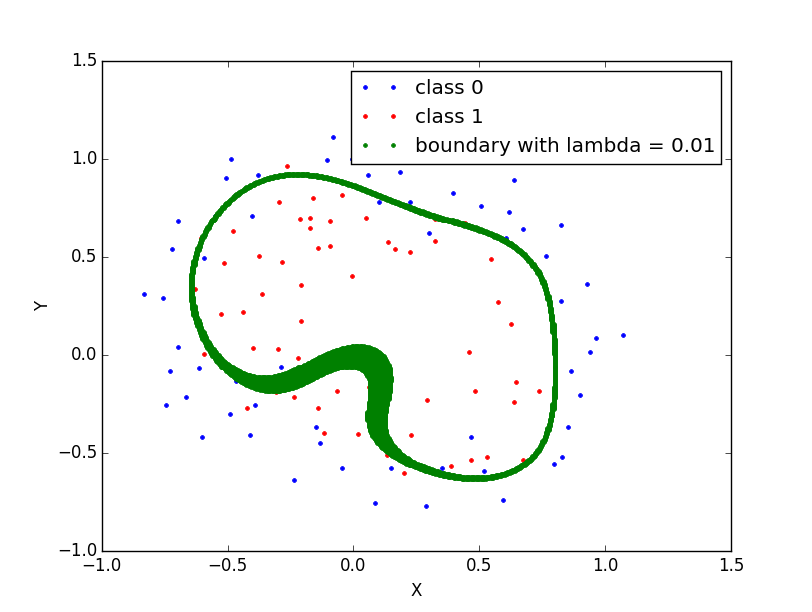
\includegraphics[scale=0.35]{lambda_good.png}
	\caption{$\lambda = 0.01$}
\end{figure}
\newpage
\section*{Exercise 6.5}
a) This is possible becuase this is essentially an OR-function which is possible to compute with a single layer perceptron.\\
Consider the sigmoid activation function $g(x)$. Our input is [1 $x_1$ $x_2$], where 1 is the bias term and $x_1$ if they have helped an old person and $x_2$ is if they have given food to a beggar. Thus, we have the weight vector [$w_1$ $w_2$ $w_3$]$^T$. If we chose our weight vector to be [-10 20 20], our input for the sigmoid $g(x)$ becomes $g(-10 + 20 x_1 + 20 x_2)$ and we can model our OR-function:
\begin{center}
  \begin{tabular}{ c | c | c }
   $x_1$ & $x_2$ & $g(x)$ \\ \hline
    0 & 0 & $g(-10) \approx 0$ \\
    0 & 1 & $g(10) \approx 1$ \\
    1 & 0 & $g(10) \approx 1$ \\
    1 & 1 & $g(30) \approx 1$
  \end{tabular}
\end{center}

b) This is also possible with a single layer perceptron, as this is essentially the AND-function.\\
Consider the sigmoid activation function $g(x)$. Our input is [1 $x_1$ $x_2$], where 1 is the bias term and $x_1$ if they have picked their nose and $x_2$ is if they didn't finish their food. Thus, we have the weight vector [$w_1$ $w_2$ $w_3$]$^T$. If we chose our weight vector to be [-30 20 20], our input for the sigmoid $g(x)$ becomes $g(-30 + 20 x_1 + 20 x_2)$ and we can model our AND-function:
\begin{center}
  \begin{tabular}{ c | c | c }
   $x_1$ & $x_2$ & $g(x)$ \\ \hline
    0 & 0 & $g(-30) \approx 0$ \\
    0 & 1 & $g(-10) \approx 0$ \\
    1 & 0 & $g(-10) \approx 0$ \\
    1 & 1 & $g(10) \approx 1$
  \end{tabular}
\end{center}

c) This can however cannot be modeled with a single layer perceptron, as this is essentially the XOR-Function, which needs at least one more layer to be computable. A single layer perceptron cannot compute the XOR function, because the bias can be chosen such that the activation function becomes 1 when one of the inputs is true but as soon as one becomes true, adding both will be true as well (see OR-function as example). Thus, we need another layer which distuinguishes between true outputs of the first layer.

\end{document}



